\documentclass[12pt,a4paper]{article}
\usepackage[utf8]{inputenc}
\usepackage{amsmath}
\usepackage{amsfonts}
\usepackage{amssymb}
\usepackage{graphicx}
\author{José Antonio García-Hernández}
\title{On Bogomoln'yi's coaxial solutions}
\begin{document}
\maketitle

In Ref.\ \cite{bogo1975}, Bomomoln'yi studies the stability of several types of topological defects. In particular, section 3 and 4 refers to the vortex line or cosmic string. He says that the vortex solution is stable unless $|n|>1$ and $\beta>1$, where $\beta = \frac{2\lambda}{n^2} = \frac{m_{\Phi}}{m_A}$, with $m_{\Phi}$ and $m_A$ are the masses of the scalar and vector fields, respectively.

He then presents the plot in Figure \ref{fig:bogo}, where he shows the profile of the scalar field $\Phi$ for values of $n$ and $\beta$. However, he did not specify the values for $v$ and $\lambda$. 

Clearly, they are coaxial solutions. He says that this coaxial behaviour is always present if the vortex is unstable. 

However, I solved the system of equations for one scalar field and the gauge field with the same parameters and did not find the coaxial behaviour. These plots are shown in figures \ref{fig:a} and \ref{fig:b}.



%\begin{figure}
%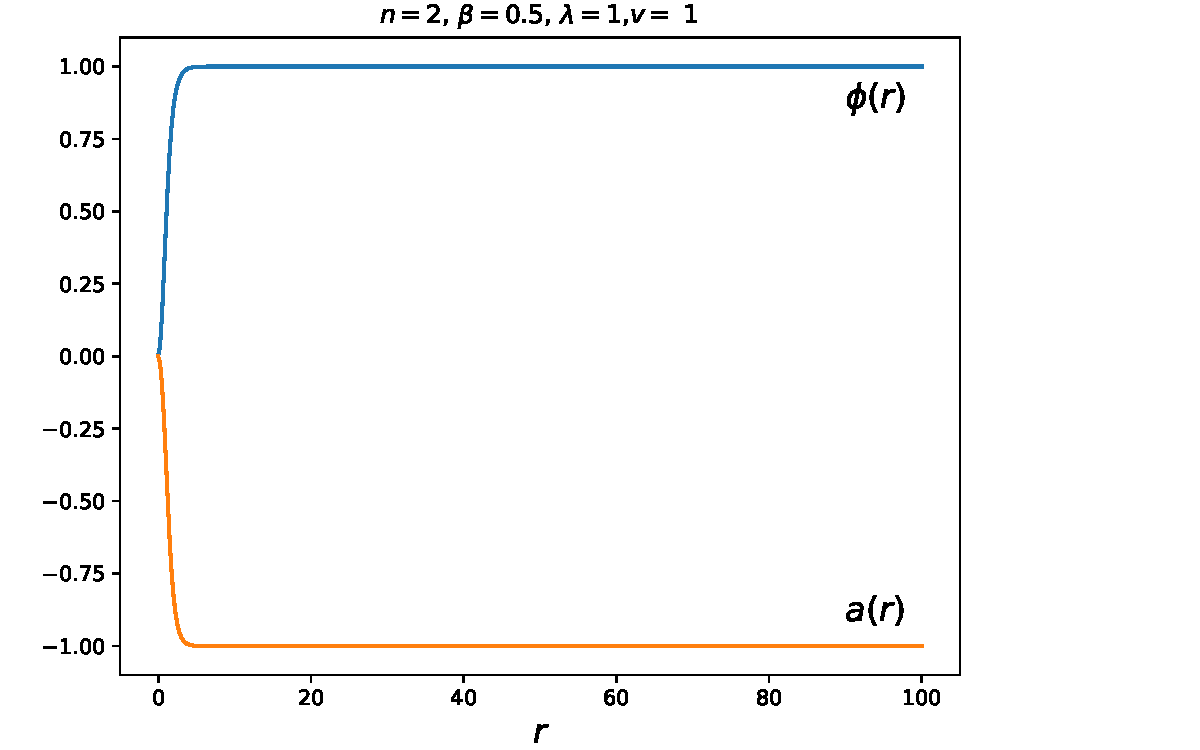
\includegraphics[scale=0.8]{n2b05l1v1.pdf}
%\caption{$n=2,\ \beta = 0.5,\ \lambda = 1,\ v = 1$.}
%\end{figure}


\begin{figure}
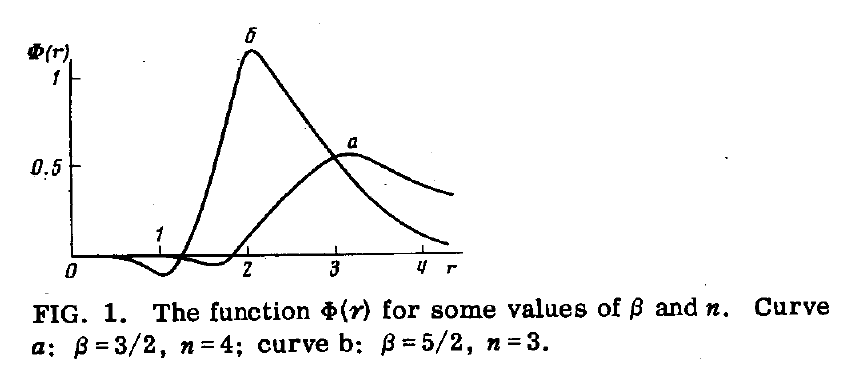
\includegraphics[scale=0.5]{bogo.png}
\caption{Bogomoln'yi's solutions.}
\label{fig:bogo}
\end{figure}

\begin{figure}
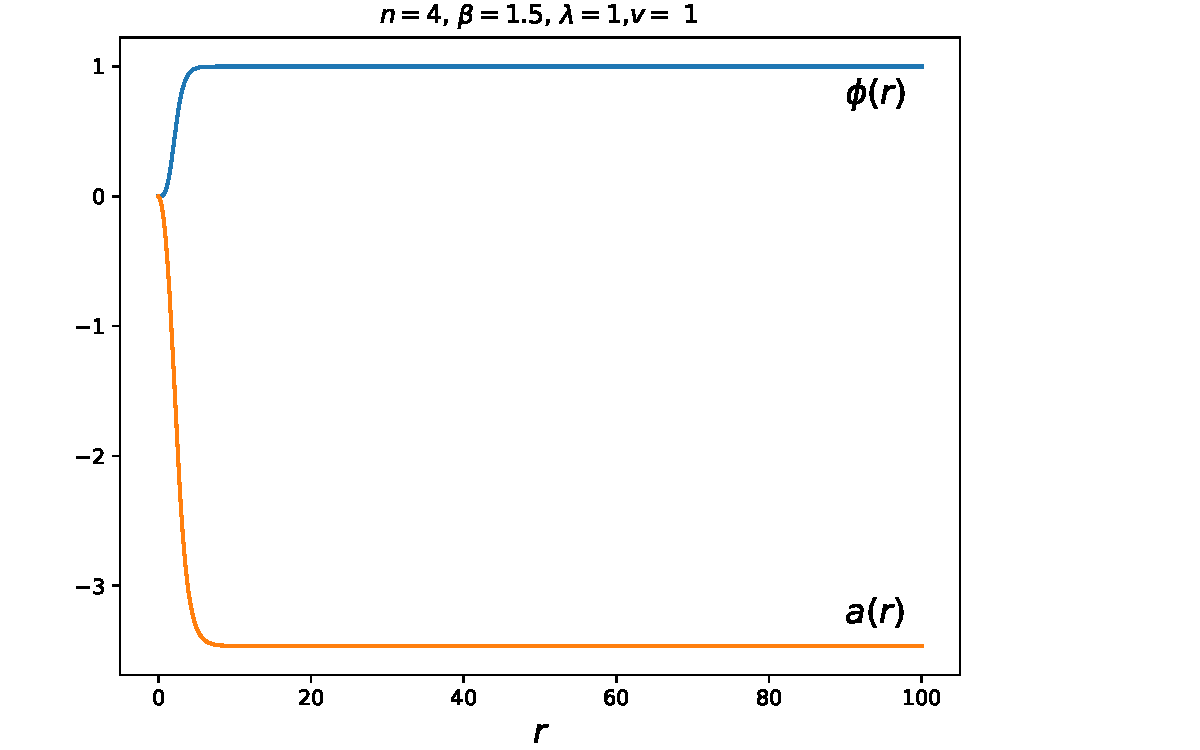
\includegraphics[scale=0.8]{n4b15l1v1.pdf}
\caption{$n=4,\ \beta = 1.5,\ \lambda = 1,\ v = 1$.}
\label{fig:a}
\end{figure}

\begin{figure}
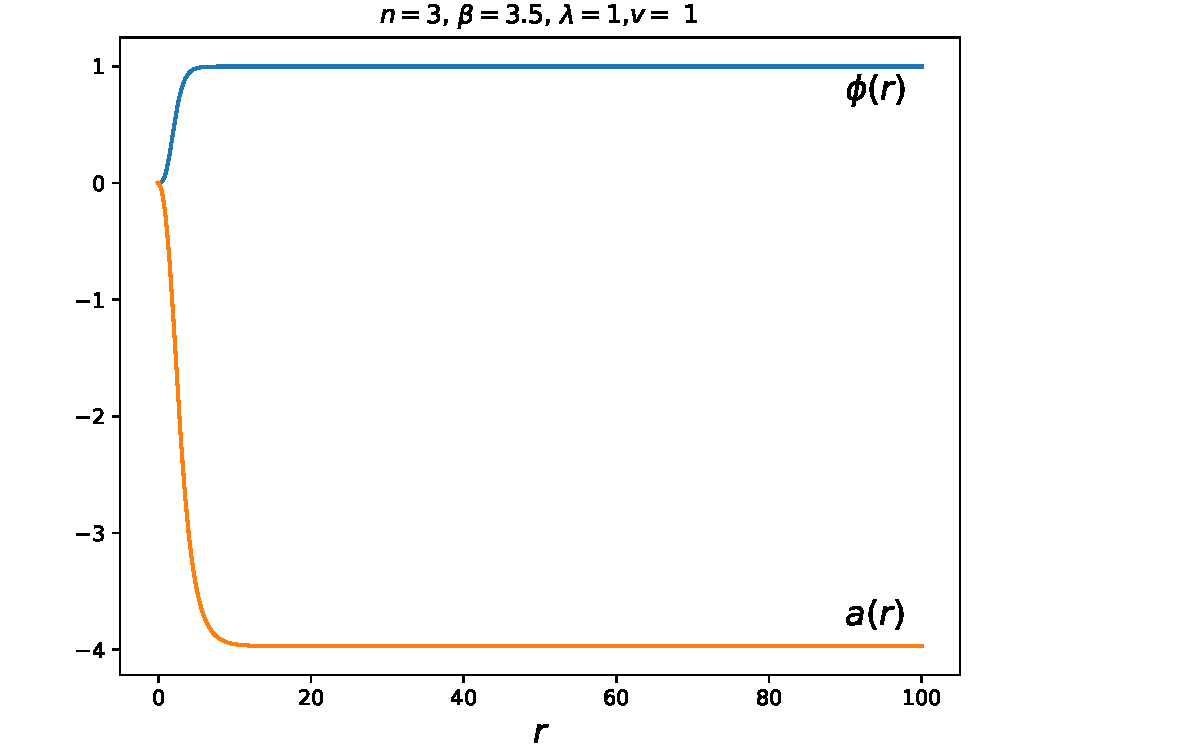
\includegraphics[scale=0.8]{n3b35l1v1.pdf}
\caption{$n=3,\ \beta = 3.5,\ \lambda = 1,\ v = 1$.}
\label{fig:b}
\end{figure}


\begin{thebibliography}{9}
\bibitem{bogo1975} Bogomoln'yi E. B. The stability of classical solutions. \emph{L. D. Landau Theoretical Physics Institute}. 24, (1975) 861-870.

\end{thebibliography}

\end{document}